%\documentclass[10pt,handout,compress,professionalfont]{beamer}
\documentclass[10pt,compress,professionalfont]{beamer}



\usepackage[latin1]{inputenc}
\usepackage{graphicx}
%\usepackage{pgf}

\usepackage{pstricks} 
\usepackage{pstricks-add} 
\usepackage{pst-plot} 
\usepackage{pst-text,pst-node,pst-tree} 

\usepackage{beamerthemeAmsterdam} 

%\hypersetup{pdfstartview={FitH}}


\setbeamertemplate{navigation symbols}{}
%\usetheme{Warsaw}
%\usecolortheme{beaver}
%\usefonttheme{structuresmallcapsserif}


\title[Point-Based Color Bleeding With Volumes]{PCBEX:\\Point-Based Color Bleeding With Volumes\\Thesis Defense}
\author{Christopher James Gibson}
\institute{California Polytechnic University\\CSC Department}
\date{June 9, 2011}

\setcounter{tocdepth}{1}

\begin{document}

\AtBeginSection[]
{
  \begin{frame}<beamer>
    \frametitle{Outline}

    \begin{columns}
        \begin{column}{0.65\textwidth}
            \tableofcontents[currentsection,currentsubsection,hideallsubsections]
        \end{column}
        \begin{column}{0.35\textwidth}
                \vspace{-9mm}
                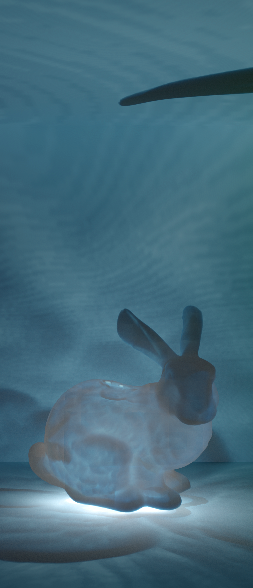
\includegraphics[height=90mm]{../img/bunny_glow_crop2}
        \end{column}
    \end{columns}
  \end{frame}
}




%%----------------------------------------------------------------------  TITLE
\begin{frame}

    \titlepage

\end{frame}




%%-------------------------------------------------------------------  SCHEDULE
\begin{frame}{Schedule}


    \begin{columns}
        \begin{column}{0.5\textwidth}
            \tableofcontents[hideallsubsections]
        \end{column}
        \begin{column}{0.5\textwidth}
            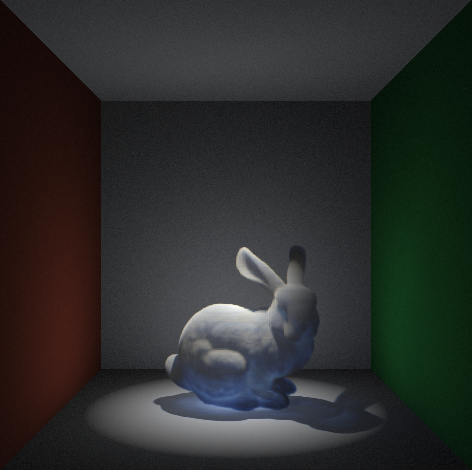
\includegraphics[width=\textwidth]{../img/spot_top_crop}
        \end{column}
    \end{columns}

\end{frame}




\section{Introduction}
%%---------------------------------------------------------------  INTRODUCTION
\begin{frame}{Graphics Intro}

    \begin{columns}
        \begin{column}{0.65\textwidth}
            {\bf Rendering} is the process of producing 2D images from a 3D scene description\\
            \vspace{8mm}
            At its core, all of {\bf computer graphics} is the visualization of how light interacts in these scenes\\
            \vspace{8mm}
            Modelling physically correct light interactions can get extremely computationally expensive\\
        \end{column}
        \begin{column}{0.35\textwidth}
                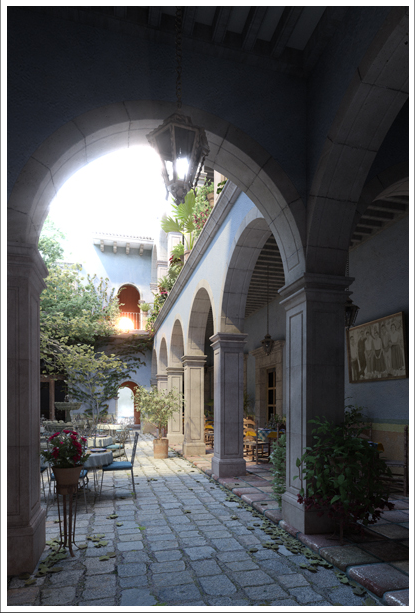
\includegraphics[width=\textwidth]{../img/external/spanish}\\
                \centering{\scriptsize\textit{(image source: Matt Pharr)}}
        \end{column}
    \end{columns}

\end{frame}




\subsection{Global Illumination}
%%--------------------------------------------  BACKGROUND: GLOBAL ILLIMUNATION
\begin{frame}{Global Illumination Introduction}

    Light's interaction with various materials and mediums is complex and beautiful\\
    \vspace{6mm}
    Light does not simply hit surfaces, but bounces and passes through them as well\\
    \vspace{4mm}

    \centering{
        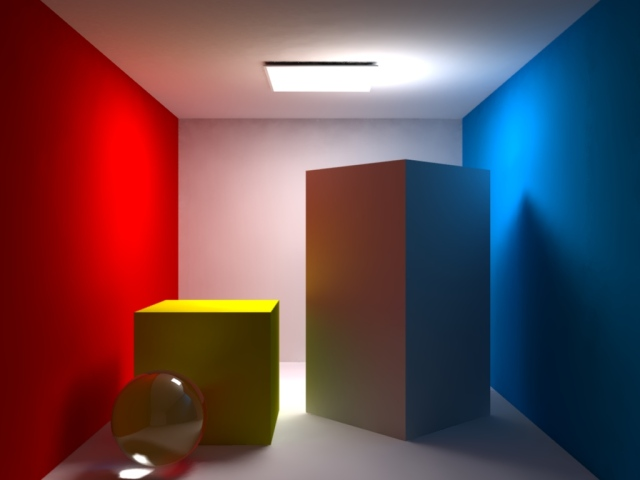
\includegraphics[width=0.55\textwidth]{../img/external/global_illumination}\\
        \scriptsize\textit{(image source: cgtutorials.com)}
    }

\end{frame}




\subsection{Global Illumination}
%%--------------------------------------------  BACKGROUND: GLOBAL ILLIMUNATION
\begin{frame}{Global Illumination}

    \begin{columns}
        \begin{column}{0.65\textwidth}
            {\bf Global Illumination} represents the set of algorithms that estimate complex lighting systems\\
            \vspace{8mm}
            The results lead to richer, more realistic images\\

        \end{column}
        \begin{column}{0.35\textwidth}
            \vspace{-8mm}
            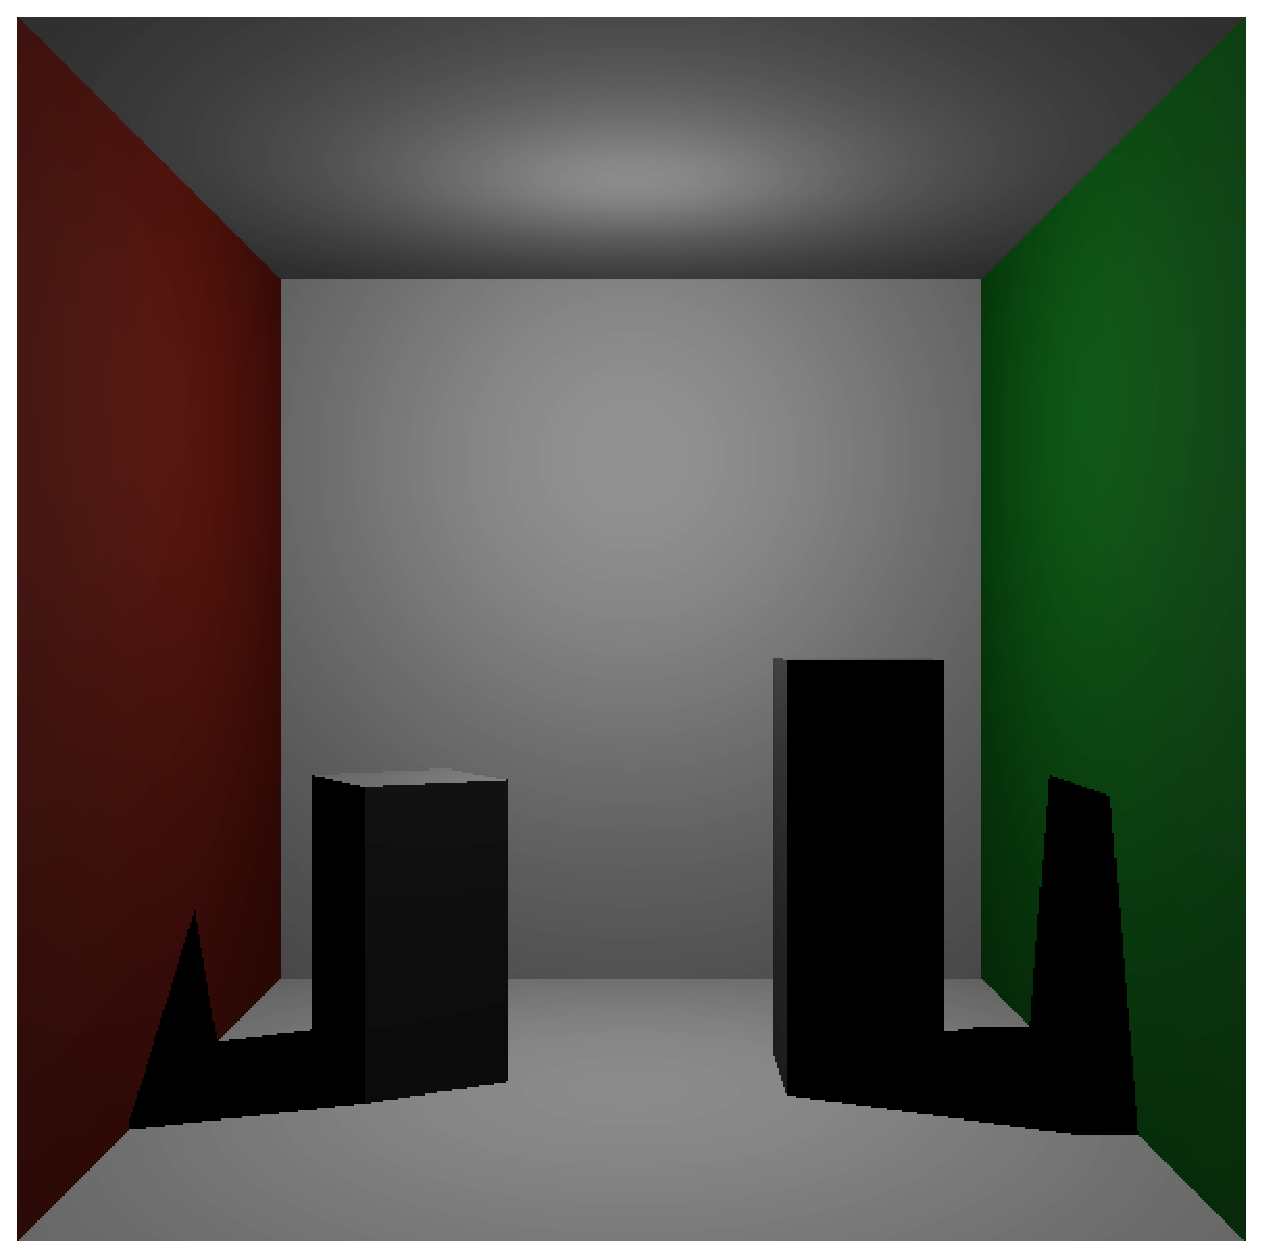
\includegraphics[width=\textwidth]{../img/boxes_noindirect}\\
            {\centering\scriptsize Direct Lighting\\}
            \vspace{2mm}
            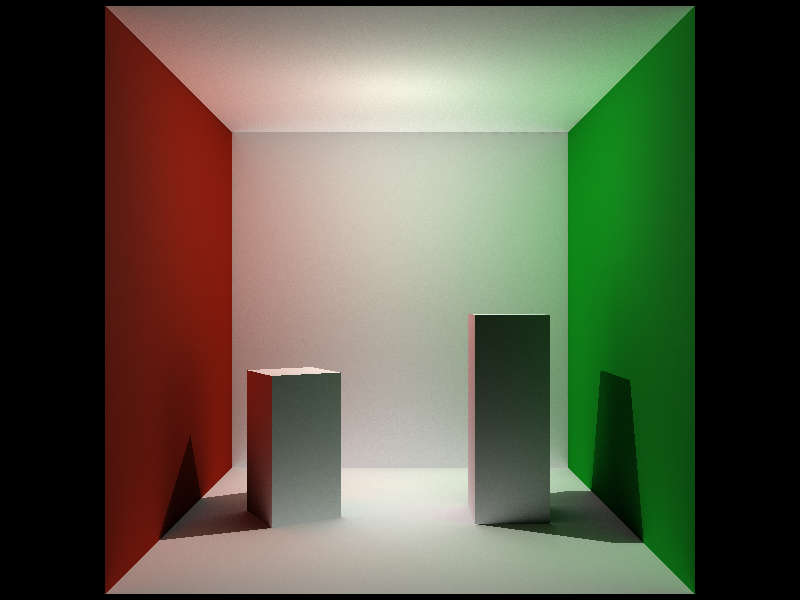
\includegraphics[width=\textwidth]{../img/indirect_box_high}\\
            {\centering\scriptsize Direct Lighting \& Global Illumination\\}
        \end{column}
    \end{columns}

\end{frame}




\subsection{Point-Based Color Bleeding}
%%------------------------------------------------  BACKGROUND: VOLUME LIGHTING
\begin{frame}{Point-Based Color Bleeding (PCB)}


    \begin{columns}
        \begin{column}{0.65\textwidth}
            Cheap, approximate global illumination effects using color bleeding\\
            \vspace{8mm}
            Utilizes direct light point cloud representation of scene's direct lighting\\
            \vspace{8mm}
            Already used heavily in production due to its performance advantages

        \end{column}
        \begin{column}{0.35\textwidth}
            \vspace{-4mm}
            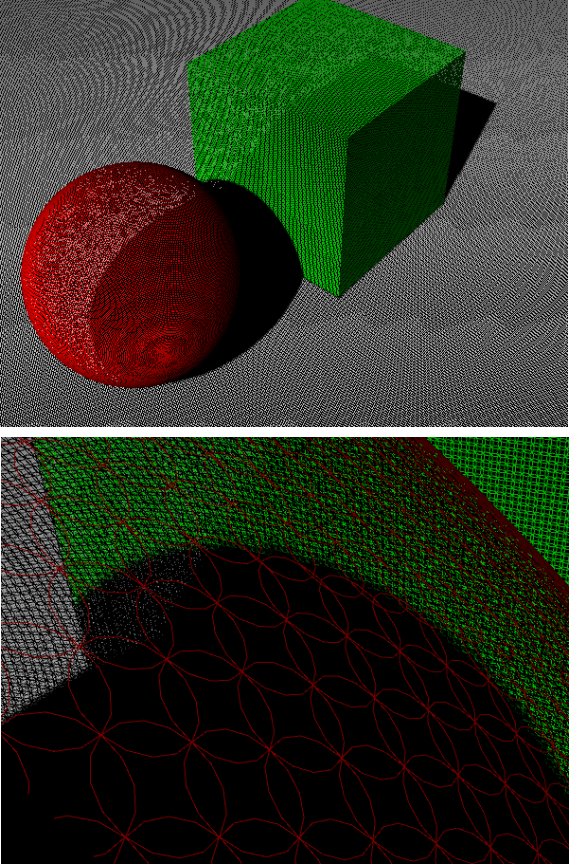
\includegraphics[width=\textwidth]{../img/external/pcb}\\
            \centering{\scriptsize Surfels in PCB\\\textit{(image source: Per Christensen)}}
        \end{column}
    \end{columns}

\end{frame}




\subsection{Volume Rendering}
%%--------------------------------------------  BACKGROUND: GLOBAL ILLIMUNATION
\begin{frame}{Volume Rendering}

    \begin{columns}
        \begin{column}{0.5\textwidth}
            {\bf Volumes} \textit{(or participating media)} represent:
            \begin{itemize}
                \item Fog
                \item Smoke
                \item Water
                \item Clouds
                \item Other Mediums...
            \end{itemize}

        \end{column}
        \begin{column}{0.5\textwidth}
            Better for visualizing three-dimensional datasets\\
            \vspace{4mm}
            Important to simulate and light properly for film, entertainment \& medical uses\\
            \vspace{4mm}
            Very computationally expensive \\ 
        \end{column}
    \end{columns}
        \centering{
        \vspace{4mm}
        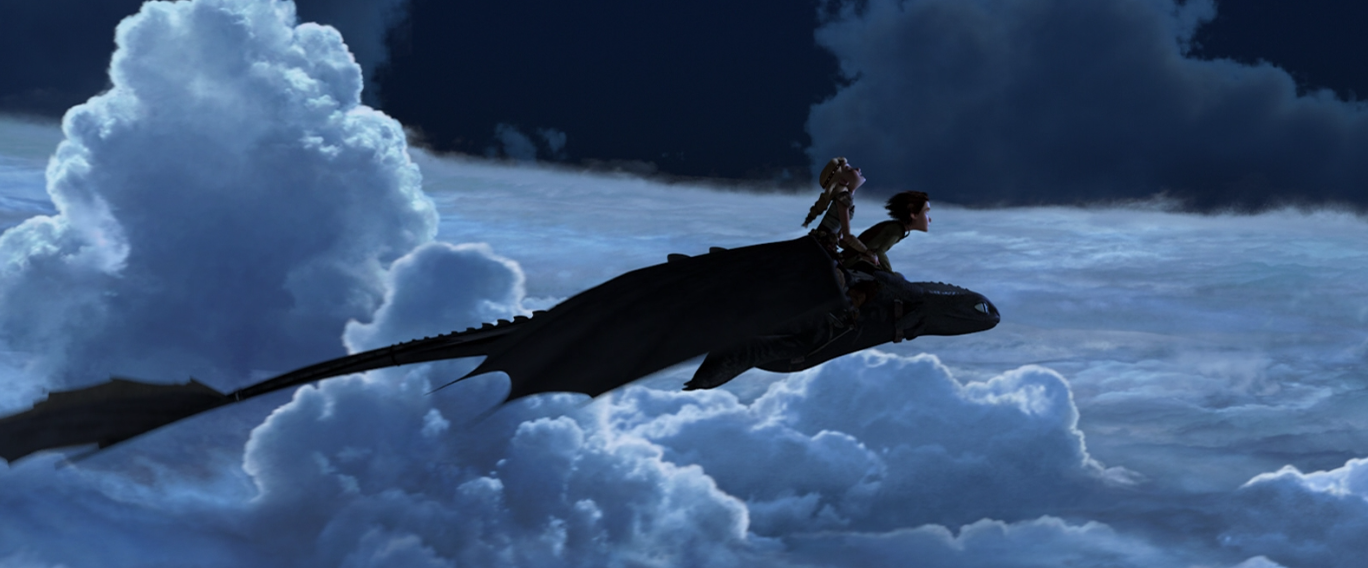
\includegraphics[width=80mm]{../img/external/smoke_dwa_2}\\
        \scriptsize\textit{(image source: DreamWorks Animation)}
        }

\end{frame}




\subsection{Motivation}
%%------------------------------------------  RELATED WORK: GLOBAL ILLIMUNATION
\begin{frame}{Motivation}

    \begin{columns}
        \begin{column}{0.35\textwidth}
            {\centering 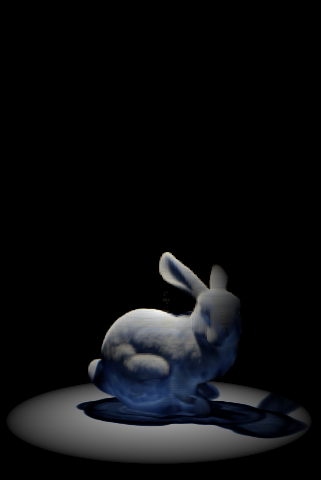
\includegraphics[width=\textwidth]{../img/bunny_spot_sad}\\}

        \end{column}
        \begin{column}{0.65\textwidth}
            Complex volume lighting algorithms are computationally expensive and complex\\
            \vspace{8mm}
            Most GA algorithms do not include volume contributions\\
            
        \end{column}
    \end{columns}
\end{frame}




\subsection{Goals}
%%------------------------------------------  RELATED WORK: GLOBAL ILLIMUNATION
\begin{frame}{Goals}

    \begin{columns}
        \begin{column}{0.5\textwidth}

            \vspace{-4mm}
            \begin{itemize}
                \item Modify existing PCB in order to include volumetric lighting\\ \vspace{2mm}
                \item Accurately model scatter, absorption and lighting properties\\ \vspace{2mm}
                \item Modify volume integration algorithm to add scatter-in effects\\ \vspace{2mm}
                \item Return comparable results with shorter overall runtimes
            \end{itemize}
        \end{column}
        \begin{column}{0.5\textwidth}
            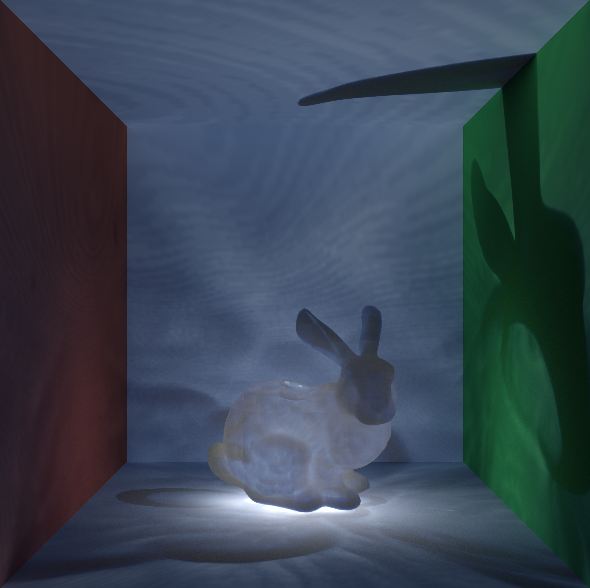
\includegraphics[width=\textwidth]{../img/bunny_glow}
        \end{column}
    \end{columns}

\end{frame}




\section{Related Work}
\subsection{Global Illumination}
%%------------------------------------------  RELATED WORK: GLOBAL ILLIMUNATION
\begin{frame}{Related Works}


    \begin{columns}
        \begin{column}{0.45\textwidth}

            Global illumination is a heavy field of research in computer graphics.\\
            \vspace{8mm}
            Involves many prominent technologies and algorithms:\\
            \vspace{2mm}
            \begin{itemize}
                \item Photon Mapping\\
                \vspace{2mm}

                \item Radiometry/Radiosity\\
                \vspace{2mm}

                \item Precomuted Light Transport\\
            \end{itemize}

        \end{column}
        \begin{column}{0.55\textwidth}
            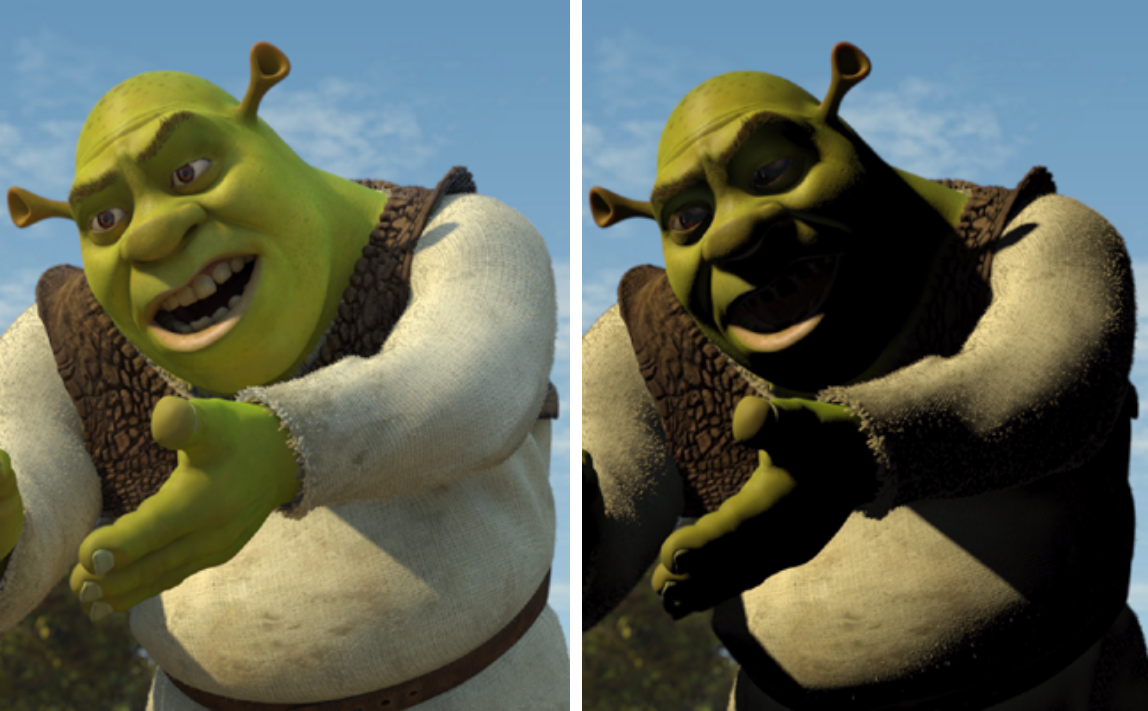
\includegraphics[width=\textwidth]{../img/external/shrek}\\
            \centering{\scriptsize Complex scene with \& without global illumination\\\textit{(image source: DreamWorks Animation)}}
        \end{column}
    \end{columns}

\end{frame}




%%------------------------------------------  RELATED WORK: GLOBAL ILLIMUNATION
\begin{frame}{Related Works: Point-Based Color Bleeding}



    \begin{columns}
        \begin{column}{0.7\textwidth}

    Point-Based Approximate Color Bleeding by Per Christensen.\\
    \vspace{6mm}

    Subset of scene geometry is thoroughly sampled, creating point cloud stored in an octree.\\
    \vspace{6mm}

    Point cloud is sampled to determine incoming radiance.

    \vspace{4mm}
    {\centering
    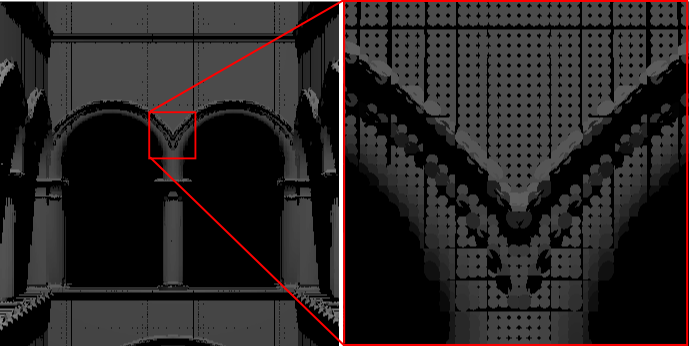
\includegraphics[width=50mm]{../img/pcloud}\\
    {\centering\scriptsize Point cloud representation\\}
    }

        \end{column}
        \begin{column}{0.3\textwidth}
            {\centering
            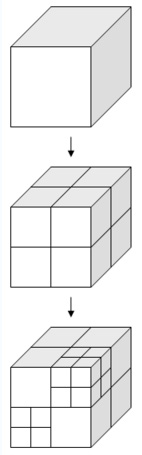
\includegraphics[height=50mm]{../img/external/octree}\\
            }
            {\centering\scriptsize Octree subdivision\\}
        \end{column}
    \end{columns}

\end{frame}




%%------------------------------------------  RELATED WORK: GLOBAL ILLIMUNATION
\begin{frame}{Related Works: Photon Mapping}

    \begin{columns}
        \begin{column}{0.5\textwidth}

    \vspace{-10mm}

    Photons cast from lights interact with the scene.  At each hit, a photon can:
    
    \begin{itemize}
        \item Bounce\\
        \vspace{2mm}

        \item Pass Through\\
        \vspace{2mm}

        \item Be Absorbed\\
    \end{itemize}

        \end{column}
        \begin{column}{0.5\textwidth}
            \vspace{-4mm}
            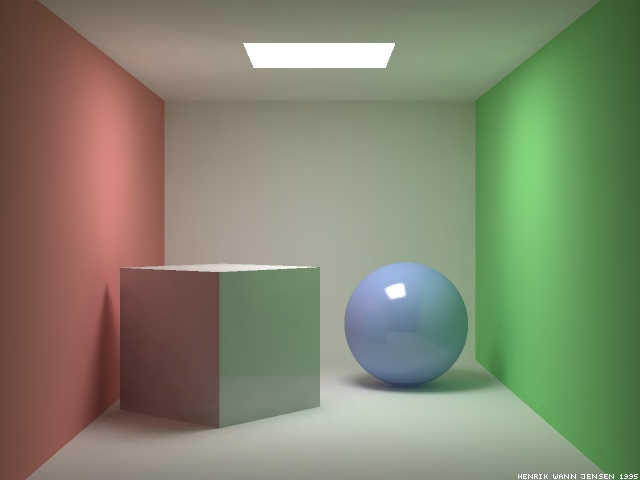
\includegraphics[width=\textwidth]{../img/external/ewr7_mcbox.jpg}\\
            \centering{\scriptsize\textit{(image source: Jensen)}}
        \end{column}
    \end{columns}
\end{frame}




\subsection{Volume Rendering}
%%---------------------------------------------  RELATED WORK: VOLUME RENDERING
\begin{frame}{Related Works: Volume Rendering}

    \begin{columns}
        \begin{column}{0.6\textwidth}

    \vspace{-10mm}

    Seminal research involved number of approaches...
    
    \begin{itemize}
        \item Polygonalization of straight voxels \textit{(boxy)}\\
        \vspace{4mm}

        \item Polygonal representation based on isosurfaces\\
        \vspace{4mm}

        \item Opacity/Color arrays \textit{(interpolation across voxels)}\\
    \end{itemize}

        \end{column}
        \begin{column}{0.4\textwidth}
            \vspace{-4mm}
            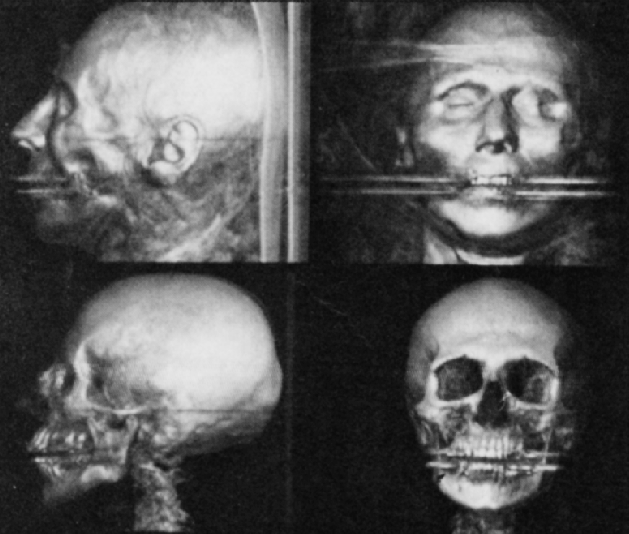
\includegraphics[width=\textwidth]{../img/external/img188}\\
            \centering{\scriptsize Renders of CT scan data\\\textit{(image source: Marc Levoy)}}
        \end{column}
    \end{columns}
\end{frame}




%%---------------------------------------------  RELATED WORK: VOLUME RENDERING
\begin{frame}{Related Works: Volume Rendering}

    \begin{columns}
        \begin{column}{0.7\textwidth}

    \vspace{-5mm}
    Multi-resolution volumes help save on memory and allow for on-demand loading\\
    \vspace{8mm}

    Occlusion techniques involving volume acceleration structures help avoid extraneous computations

        \end{column}
        \begin{column}{0.3\textwidth}
            \vspace{-4mm}
            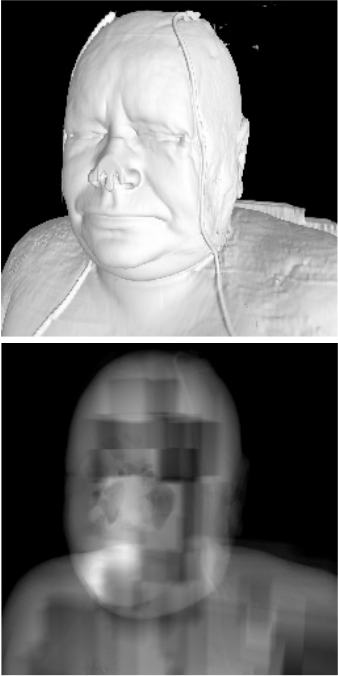
\includegraphics[width=\textwidth]{../img/external/vol_multi_res}\\
            \centering{\scriptsize Renders of CT scan data\\\textit{(image source: S. Guthe)}}
        \end{column}
    \end{columns}

\end{frame}




\section{Background}
%%-----------------------------------------------------------------  BACKGROUND
\subsection{Illumination and Light}
%%---------------------------------------------------  BACKGROUND: ILLIMUNATION
\begin{frame}{Flux and Radiance}

    {\bf Flux} is the measure of total light emitted \textit{(Watts)}

    \begin{columns}
        \begin{column}{0.6\textwidth}
            \begin{block}{Radiance Equation}
                \[
                \mathit{L} = \frac{\mathit{d^{2}\Phi}}{\mathit{dw\:dA}^\perp} = \frac{\mathit{d^{2}\Phi}}{\mathit{dw\:dA}\textup{cos}\theta}
                \]
            \end{block}
            \begin{block}{Radiance Invariance}
                \[
                    L(x \to y) = L(y \to x)
                \]
            \end{block}
        \end{column}
        \begin{column}{0.4\textwidth}
            \vspace{-5mm}
            {\centering
                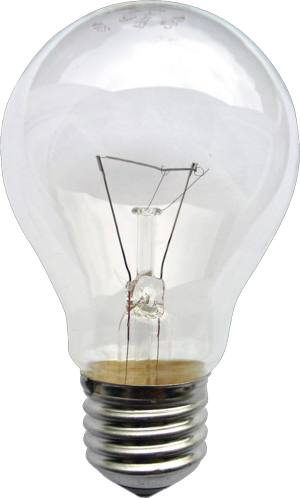
\includegraphics[width=\textwidth]{../img/external/lightbulb}\\
            }
        \end{column}
    \end{columns}


        % NOTE: Flux density per unit area, per unit solid angle
        % NOTE: dA is the projection of dA on a plane perpendicular to w
        % NOTE: radiance is incoming light power

\end{frame}




%%---------------------------------------------------  BACKGROUND: ILLIMUNATION
\begin{frame}{Irradiance}

    \begin{columns}
        \begin{column}{0.5\textwidth}
                \begin{block}{Irradiance Equation}
                    \[
                    E = \frac{d\Phi}{dA}
                    \]\\
                    \vspace{4mm}
                    {\centering Taking radiance into account:\\}
                    \[
                        \mathit{E} = \int\mathit{L}(\textup{p} \leftarrow w)\textup{cos}\theta dw
                    \]
                \end{block}
        \end{column}
        \begin{column}{0.5\textwidth}
            \vspace{-5mm}
            {\centering
            \includegraphics[width=\textwidth]{../img/diag/radiance.pdf}\\
            \scriptsize Radiance diagram\\
            }
        \end{column}
    \end{columns}


        % NOTE: Flux density per unit area, per unit solid angle
        % NOTE: dA is the projection of dA on a plane perpendicular to w
        % NOTE: radiance is incoming light power

\end{frame}




\subsection{BRDF}
%%-----------------------------------------------------------  BACKGROUND: BRDF
\begin{frame}{BRDF}

    {\centering
        {\bf B}idirectional {\bf R}eflectance {\bf D}istribution {\bf F}unction\\
        \vspace{4mm}
        Gives us a formalism for describing the reflection from a surface\\
    }

    \begin{columns}
        \begin{column}{0.55\textwidth}

            \begin{block}{Incoming Radiance from $w_i$}
            \[
                \mathit{dE}(\textup{p}, w_i) = \int\mathit{L_i}(\textup{p} \leftarrow w_i)\textup{cos}\theta_i dw_i.
            \]
            \end{block}
            \begin{block}{Incoming vs Outgoing Radiance}
            \[
                f_r(\textup{p}, w_o, w_i) =  \frac{dL_o(\textup{p},w_o)}{dE(\textup{p},w_i)}
            \]
            \end{block}

        \end{column}
        \begin{column}{0.45\textwidth}
            \vspace{10mm}
            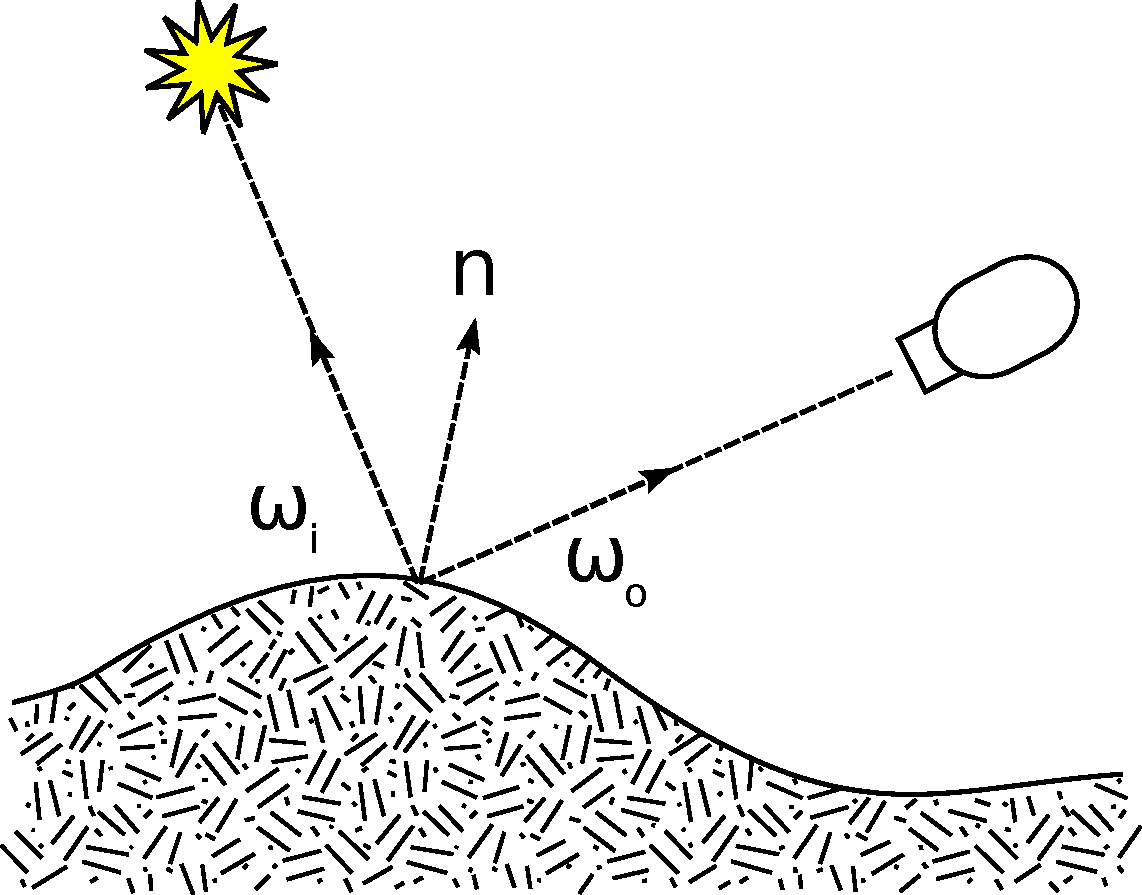
\includegraphics[width=\textwidth]{../img/external/BRDF_Diagram.pdf}\\
            \centering{\scriptsize BRDF Visualization\\\textit{(image source: Wikipedia)}}
        \end{column}
    \end{columns}
\end{frame}




\subsection{BRDF}
%%-----------------------------------------------------------  BACKGROUND: BRDF
\begin{frame}{BRDF}

    {\centering
        Note: $f_r$ is a function based on the reflection properties of the surface \\
        \vspace{4mm}
        Therefore, we can solve for $L_o$\\
    }

    \begin{block}{Incoming Radiance from $w_i$}
    \[
        \mathit{L_o}(\textup{p}, w_o) = \int{\mathbb{S}^2} \mathit{f_r}(\textup{p}, w_o, w_i)\:L_i(\textup{p}, w_i)cos\theta_i dw.
    \]
    \end{block}
    \centering{
        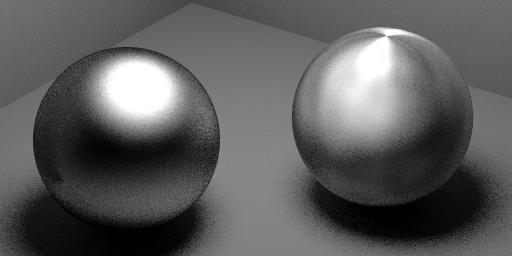
\includegraphics[width=60mm]{../img/external/brdf.jpg}\\
        {\scriptsize BRDF Visualization\\\textit{(image source: Cornell.edu)}}
    }

\end{frame}




%%-----------------------------------------------------------  BACKGROUND: BRDF
\begin{frame}{BSSRDF}
    
    {\centering
        {\bf B}idirectional {\bf S}cattering-{\bf S}urface {\bf R}eflectance {\bf D}istribution {\bf F}unction
    }
    \vspace{4mm}
    \begin{columns}
        \begin{column}{0.6\textwidth}

            Helps model the interactions of light within a surface \textit{(also known as subsurface scattering.)}\\
            \vspace{8mm}
            Far more complex than traditional BRDF evaluations.\\

            \begin{block}{Incoming vs Outgoing Radiance}
            \[
                f_r(\textup{p}_o, w_o, \textup{p}_i, w_i) =  \frac{dL_o(\textup{p}_o,w_o)}{dE(\textup{p}_i,w_i)}.
            \]
            \end{block}

        \end{column}
        \begin{column}{0.4\textwidth}
            \vspace{10mm}
            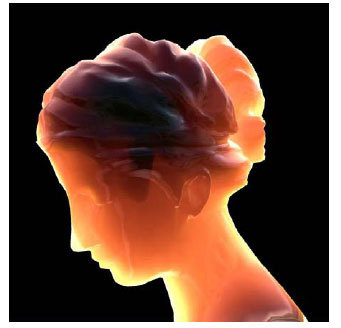
\includegraphics[width=\textwidth]{../img/external/subscat}\\
            \centering{
                \scriptsize Light scattering inside of a statue\\
                \textit{(image source: Nvidia)}
            }
        \end{column}
    \end{columns}

\end{frame}



\subsection{Volume Lighting}
%%---------------------------------------------------  BACKGROUND: ILLIMUNATION
\begin{frame}{Volume Lighting}

    \centering
    \vspace{0cm}
    \includegraphics[width=100mm]{../img/diag/vol_scatter.pdf}

\end{frame}




%%---------------------------------------------------  BACKGROUND: ILLIMUNATION
\begin{frame}{Volume Lighting - Absorption}

    \begin{columns}
        \begin{column}{0.55\textwidth}

            \begin{block}{Absorption Equation}
                \[
                    e^{-\int_{0}^{d}\sigma_{a} (p+t\mathit{w},\mathit{w})d\mathit{t}}
                \]
            \end{block}
            \vspace{8mm}
            Some particles will absorb light passing through. Also known as extinction.\\
            \vspace{8mm}
            Most commonly seen in smoke or ash clouds

        \end{column}
        \begin{column}{0.45\textwidth}
            \vspace{10mm}
            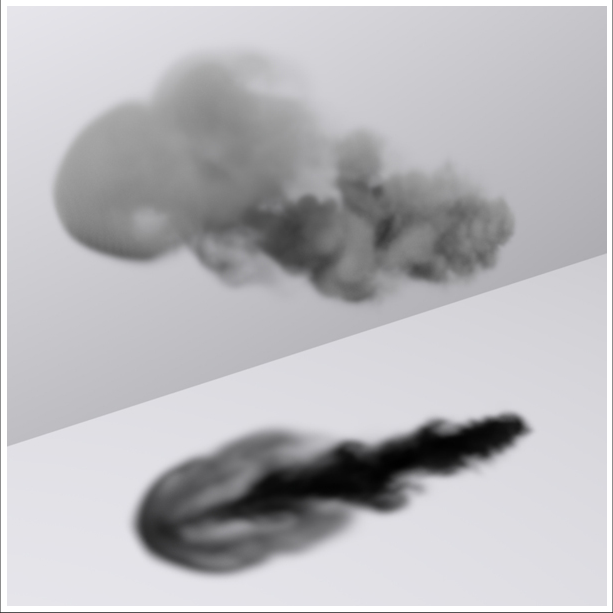
\includegraphics[width=\textwidth]{../img/external/scatter}\\
            \centering{\scriptsize Extinction in a volume\\\textit{(image source: Matt Pharr)}}
        \end{column}
    \end{columns}

\end{frame}




%%---------------------------------------------------  BACKGROUND: ILLIMUNATION
\begin{frame}{Volume Lighting - Scatter}

    \begin{columns}
        \begin{column}{0.55\textwidth}

            \begin{block}{Scatter Out Equation}
                \[
                    d\mathit{L}_{o}(\textup{p},w) = -\sigma_{s}(\textup{p},w) \mathit{L}_{i}(\textup{p},-w)dt
                \]
            \end{block}
            \vspace{8mm}
            Scatter out is the reduction of light along a path as it is scattered by the participating media.\\
            \vspace{8mm}
            Clouds exemplify high scatter and low absorption.

        \end{column}
        \begin{column}{0.45\textwidth}
            \vspace{10mm}
            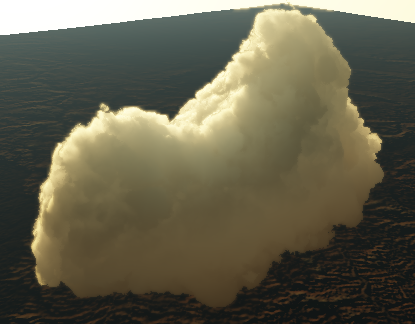
\includegraphics[width=\textwidth]{../img/external/cloud}\\
            \centering{\scriptsize Scatter in a volume\\\textit{(image source: blenderartists.org)}}
        \end{column}
    \end{columns}

\end{frame}




%%---------------------------------------------------  BACKGROUND: ILLIMUNATION
\begin{frame}{Volume Lighting- Transmittance}


    \begin{columns}
        \begin{column}{0.5\textwidth}

            \begin{block}{Transmittance Equation}
                \[
                    T_{r}(\textup{p} \to \textup{p}') = e^{-\int_{0}^{d}\sigma (p+t\mathit{w},\mathit{w})d\mathit{t}}.
                \]
            \end{block}
            \vspace{5mm}

            Evaluates how much light was left unabsorbed after passing through the volume.\\
            \vspace{5mm}
            Helps us estimate how much light bleeds through volumes from behind.

%            \begin{block}{Source Normalization}
%                \[
%                    \int_{\mathbb{S}^2}phase(w \to w')\textup{d}w' = 1.
%                \]
%            \end{block}

        \end{column}
        \begin{column}{0.5\textwidth}
            \vspace{10mm}
            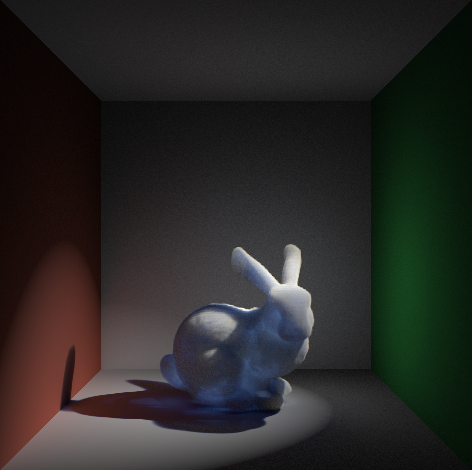
\includegraphics[width=\textwidth]{../img/bunny_spot/spot_right_new}\\
            {\centering\scriptsize Light passing through the bunny volume\\}
        \end{column}
    \end{columns}

\end{frame}




%%---------------------------------------------------  BACKGROUND: ILLIMUNATION
\begin{frame}{Volume Lighting - Scatter-In}

    \begin{block}{Scatter-In Equation}
        \[
            \mathit{S}(\textup{p},w) = \mathit{L}_{\textup{ve}}(\textup{p},w) + \sigma_{\textup{s}}(\textup{p}, w) \int_{\mathbb{S}^2} phase(\textup{p}, -w' \to w) L_{i}(\textup{p},w')\textup{d}w'.
        \]
    \end{block}
    {\centering
    \vspace{8mm}
    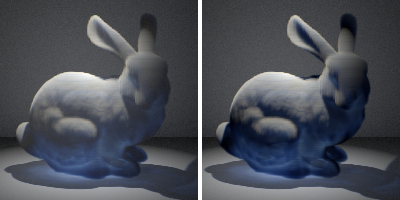
\includegraphics[width=60mm]{../img/inscat_comp}\\
    {\centering\scriptsize Scatter-in \textit{(left)} and only direct lighting via transmittance \textit{(right)}\\}
    }

\end{frame}




%%---------------------------------------------------  BACKGROUND: ILLIMUNATION
\begin{frame}{Volume Lighting- Phase Functions}


    \begin{columns}
        \begin{column}{0.5\textwidth}

            \begin{block}{Phase Function}
                Described as $phase(w \to w')$
            \end{block}
            \vspace{5mm}

            Describes the probability that light will scatter in any given direction.\\
            \vspace{5mm}
            Used to estimate total scatter-in contribution.

%            \begin{block}{Source Normalization}
%                \[
%                    \int_{\mathbb{S}^2}phase(w \to w')\textup{d}w' = 1.
%                \]
%            \end{block}

        \end{column}
        \begin{column}{0.5\textwidth}
            \vspace{10mm}
            \includegraphics[width=\textwidth]{../img/diag/phase_func_sm}\\
            {\centering\scriptsize Phase function distribution\\}
        \end{column}
    \end{columns}

\end{frame}




\subsection{Monte Carlo Integration}
%%-----------------------------------------------  BACKGROUND WORK: MONTE CARLO
\begin{frame}{Monte Carlo Integration}


    \begin{columns}
        \begin{column}{0.6\textwidth}

    \vspace{-10mm}
    Monte Carlo methods allow estimation of complex systems through use of probability functions and random numbers.\\
    \vspace{8mm}

    Most useful to us is Monte Carlo Integration.

        \end{column}
        \begin{column}{0.4\textwidth}
            \vspace{-4mm}
            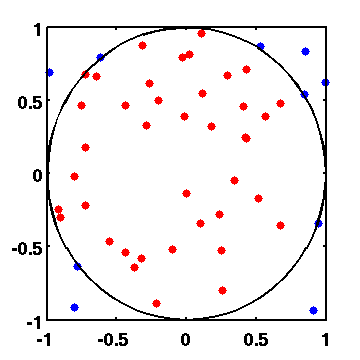
\includegraphics[width=\textwidth]{../img/external/MonteCarloIntegrationCircle}\\
            {\centering\scriptsize Randomly sampling a circle\\}
        \end{column}
    \end{columns}

\end{frame}




\section{PCB Extension Algorithm}
\subsection{PCB Algorithm Overview}
%%--------------------------------------------------------------  PCB EXTENSION
\begin{frame}{Point-Based Color Bleeding}



    \begin{columns}
        \begin{column}{0.6\textwidth}
            \begin{enumerate}
                \item Sample the scene and generate a point cloud
                \item Perform normal ray tracing
                \item Replace ambient estimates with a gather stage using surrounding point cloud
            \end{enumerate}
        \end{column}
        \begin{column}{0.4\textwidth}
            {\centering
                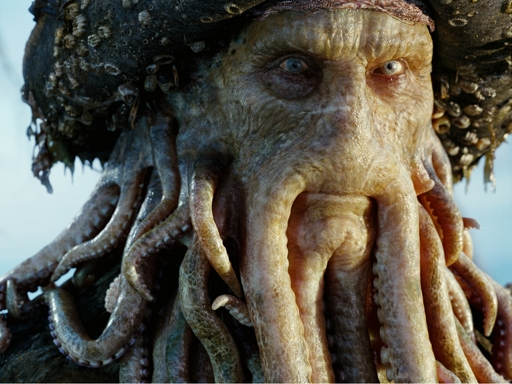
\includegraphics[width=\textwidth]{../img/external/davyjones}\\
                \scriptsize\textit{(image source: Disney)}
            }
        \end{column}
    \end{columns}
\end{frame}




\subsection{Extension Overview}
%%--------------------------------------------------------------  PCB EXTENSION
\begin{frame}{Extension Overview}

    \begin{enumerate}
        \item Sample the scene and generate a point cloud
        \item \alert{ Sample the participating media to evaluate scatter, absorbtion and direct lighting}
        \item Perform normal ray tracing
        \item Replace ambient estimates with a gather stage using surrounding point cloud \alert{using a modified traversal algorithm}
        \item \alert{ Model and scatter-in properties during volume integration}
    \end{enumerate}
    \vspace{4mm}
    {\centering
        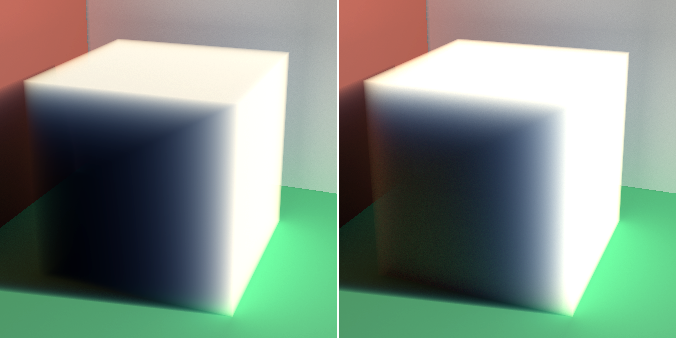
\includegraphics[width=70mm]{../img/inscat_comp2}\\
    }

\end{frame}




\subsection{Sampling the Scene}
%%--------------------------------------------------------------  PCB EXTENSION
\begin{frame}{Sampling the Scene}

    \begin{columns}
        \begin{column}{0.5\textwidth}

    \vspace{-5mm}
    Rays are cast and intersections with objects are recorded\\
    \vspace{8mm}

    Sampling "camera" is behind normal camera with wider field of view\\
    \vspace{8mm}

    \textit{Surfels} are oriented at the intersections aligned along the surface normal

        \end{column}
        \begin{column}{0.5\textwidth}
            \vspace{-4mm}
            \includegraphics[width=\textwidth]{../img/diag/surfel_samp_mod.pdf}\\
        \end{column}
    \end{columns}

\end{frame}




\subsection{Integrating Volume Data}
%%--------------------------------------------------------------  PCB EXTENSION
\begin{frame}{Sampling Volumes}

    \begin{columns}
        \begin{column}{0.5\textwidth}

    Samples are taken at discrete steps across the volume domain\\
    \vspace{8mm}

    Scatter/Absorbtion/Lighting factors are averaged within each step\\
    \vspace{8mm}

    \textit{Lvoxels} (spheres) instead of \textit{surfels}

        \end{column}
        \begin{column}{0.5\textwidth}
            \includegraphics[width=\textwidth]{../img/diag/vol_step.pdf}\\
            \vspace{-4mm}
        \end{column}
    \end{columns}

\end{frame}




\subsection{Gathering Light}
%%--------------------------------------------------------------  PCB EXTENSION
\begin{frame}{Gathering Light}

    \begin{columns}
        \begin{column}{0.5\textwidth}

    \vspace{-5mm}
    At render time, rays are cast from normal camera\\
    \vspace{8mm}

    Samples are cast from intersecting surface oriented along its normal

        \end{column}
        \begin{column}{0.5\textwidth}
            \includegraphics[width=\textwidth]{../img/diag/orthnormal.pdf}\\
            \vspace{-4mm}
        \end{column}
    \end{columns}

\end{frame}




%%--------------------------------------------------------------  PCB EXTENSION
\begin{frame}{Gathering Light}

    \begin{columns}
        \begin{column}{0.5\textwidth}

    \vspace{-5mm}
    Samples cast into point cloud "gather" light via intersection\\
    \vspace{8mm}

    Samples are returned and used to evaluate the integral over the aligned hemisphere

        \end{column}
        \begin{column}{0.5\textwidth}
            \includegraphics[height=\textwidth]{../img/diag/gather.pdf}\\
            \vspace{-4mm}
        \end{column}
    \end{columns}
    

\end{frame}




%%--------------------------------------------------------------  PCB EXTENSION
\begin{frame}{Integrating Volume Data - Scatter Out}

    \begin{columns}
        \begin{column}{0.5\textwidth}

    Gather stage remains same, no changes necessary\\
    \vspace{8mm}

    Octree must be traversed from back-to-front in order to integrate properly\\
    \vspace{8mm}

    Must keep track of transmittance during traversal

        \end{column}
        \begin{column}{0.5\textwidth}
            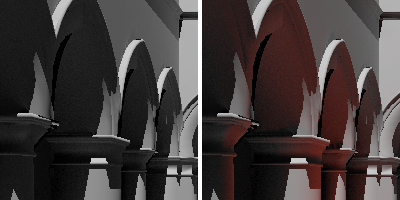
\includegraphics[width=\textwidth]{../img/compare_trad_corrected}\\
            \vspace{2mm}
            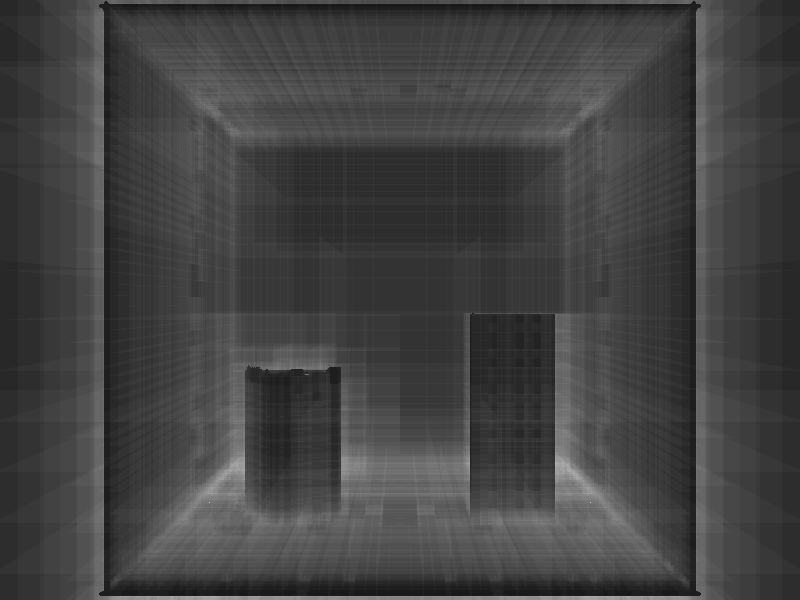
\includegraphics[width=\textwidth]{../img/testing}\\
        \end{column}
    \end{columns}

\end{frame}




%%--------------------------------------------------------------  PCB EXTENSION
\begin{frame}{Integrating Volume Data - Scatter In}

    \begin{columns}
        \begin{column}{0.5\textwidth}

            Modify integration code (normal volume rendering)\\
            \vspace{8mm}

            Add spherical sampling at each volume step\\
            \vspace{8mm}

            For increased performance, guarantee full distribution across multiple steps, not at each step

        \end{column}
        \begin{column}{0.5\textwidth}
            \includegraphics[width=\textwidth]{../img/diag/scatter_in.pdf}\\
        \end{column}
    \end{columns}

\end{frame}




\section{Results}
\subsection{Evaluation}
%%--------------------------------------------------------------------  RESULTS
\begin{frame}{Results - Environment}

    {\bf Test scene involved:}
    \begin{itemize}
        \item 60,000 triangle Sponza Atrium Model\\
        \vspace{2mm}
        \item Stanford Bunny \textit{(Volume Data)}
    \end{itemize}
    \vspace{10mm}
    {\centering
    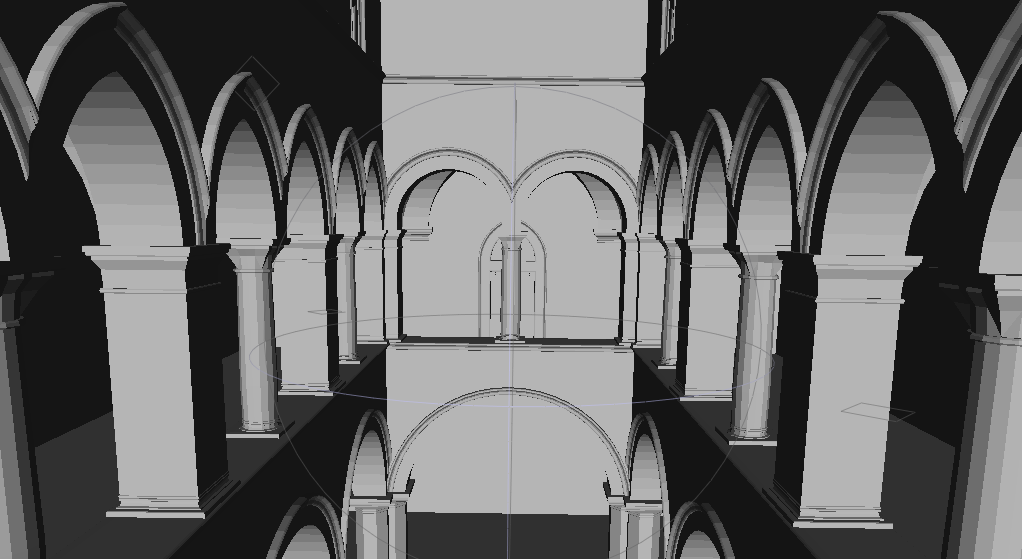
\includegraphics[width=80mm]{../img/sponza_vis}\\
    }

\end{frame}




%%--------------------------------------------------------------------  RESULTS
\begin{frame}{Results}



    \vspace{5mm}


    \begin{columns}
        \begin{column}{0.6\textwidth}
            {\bf Test run configuration:}
            \begin{itemize}
                \item Run on dual core Intel i5 3.4 GHz, 16 GB machine\\
                \vspace{2mm}
                \item 128 samples per bounce (single bounce)\\
                \vspace{2mm}
                \item 16 samples per in-scatter test\\
                \vspace{2mm}
                \item OpenMP threads split image into vertical chunks for processing\\
            \end{itemize}

        \end{column}
        \begin{column}{0.4\textwidth}

            {\centering
            
\includegraphics[width=\textwidth]{../img/threads}\\
            {\centering\scriptsize Thread distribution across the image\\}
            }
        \end{column}
    \end{columns}
\end{frame}




%%--------------------------------------------------------------------  RESULTS
\begin{frame}{Results}

    \begin{center}
    \setlength{\tabcolsep}{2pt}
    \begin{tabular}{ | l | c | c | c | }
      \hline                       
      Scene & Render Time (s) & Image Delta & Memory Overhead \\
      \hline                  
      Monte Carlo w/o PCB & 3351 sec & NONE & NONE \\
      Traditional PCB & 348 sec & 11.0\% & 390 Mb (4.0\%) \\
      Extended PCB & 397 sec & 4.8\% & 395 Mb (4.1\%)  \\
      \hline  
    \end{tabular}
    \end{center}

\end{frame}




%%-----------------------------------------------------------------  CONCLUSION
\begin{frame}[c]{}

    {\centering
    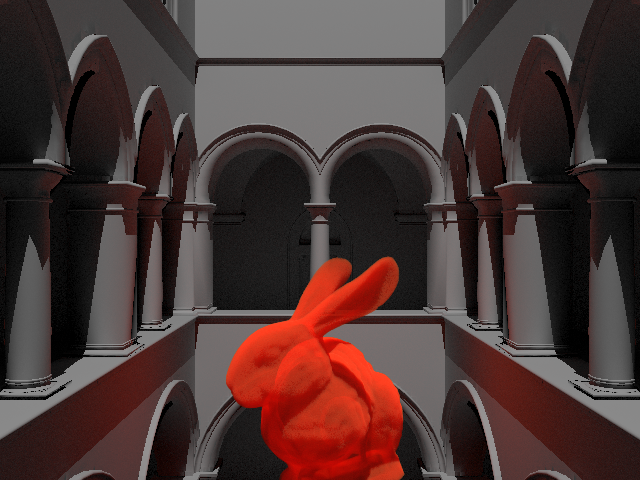
\includegraphics[width=80mm]{../img/sponza}\\
    }
    {\centering\scriptsize Sponza scene rendered with PCBEX\\}

\end{frame}




%%-----------------------------------------------------------------  CONCLUSION
\begin{frame}[c]{}

    {\centering
    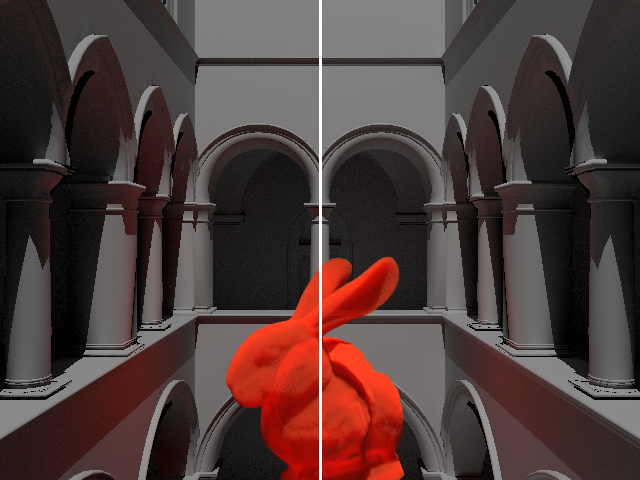
\includegraphics[width=80mm]{../img/compare}\\
    }
    {\centering\scriptsize Comparison of PCBEX results \textit{(left)} and Monte Carlo results \textit{(right)}\\}

\end{frame}




%%--------------------------------------------------------------------  RESULTS
\begin{frame}{Image Comparison}


    \begin{columns}
        \begin{column}{0.5\textwidth}
            Close-ups show drastic difference between PBC and PBCEX renders.\\
            \vspace{8mm}
            Full Monte Carlo renders differ only slightly from PCBEX renders.
        \end{column}
        \begin{column}{0.5\textwidth}

            {\centering
            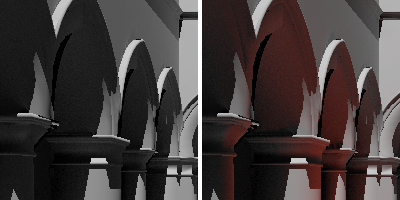
\includegraphics[width=50mm]{../img/compare_trad_corrected}\\
            {\centering\scriptsize PBC vs PBCEX\\}
            
            \vspace{5mm}

            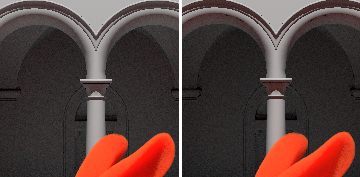
\includegraphics[width=50mm]{../img/compare1_corrected}\\
            {\centering\scriptsize Monte Carlo vs PBCEX\\}
            }
        \end{column}
    \end{columns}


\end{frame}




%%-----------------------------------------------------------------  CONCLUSION
\begin{frame}[c]{}

    \begin{columns}
        \begin{column}{0.5\textwidth}
            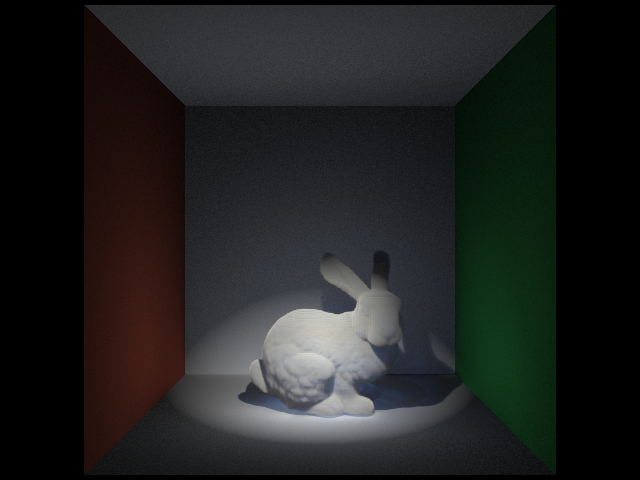
\includegraphics[width=\textwidth]{../img/bunny_spot/spot_front}\\
            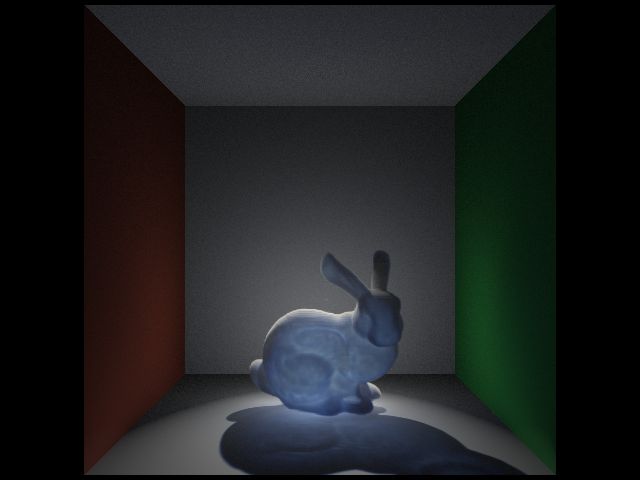
\includegraphics[width=\textwidth]{../img/bunny_spot/spot_behind}\\

        \end{column}
        \begin{column}{0.5\textwidth}
            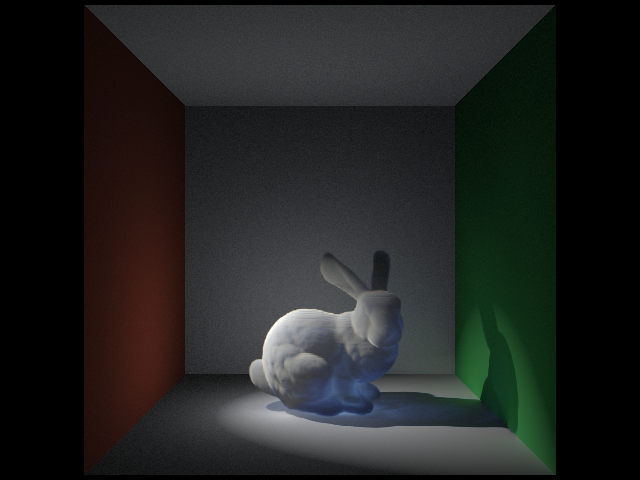
\includegraphics[width=\textwidth]{../img/bunny_spot/spot_left}\\
            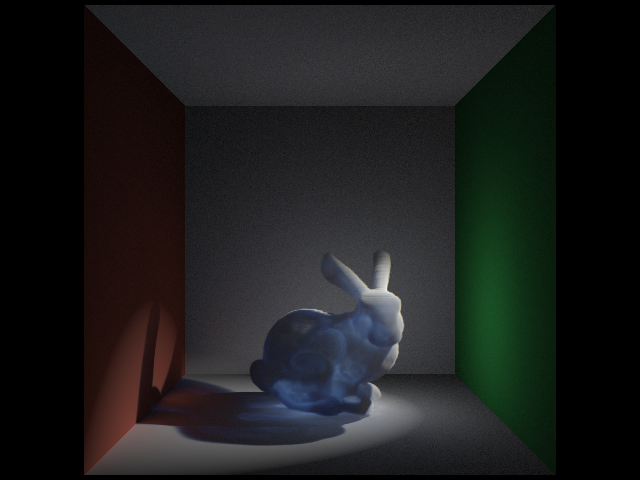
\includegraphics[width=\textwidth]{../img/bunny_spot/spot_right}\\
        \end{column}
    \end{columns}

\end{frame}




%%-----------------------------------------------------------------  CONCLUSION
\begin{frame}[c]{}

    {\centering
    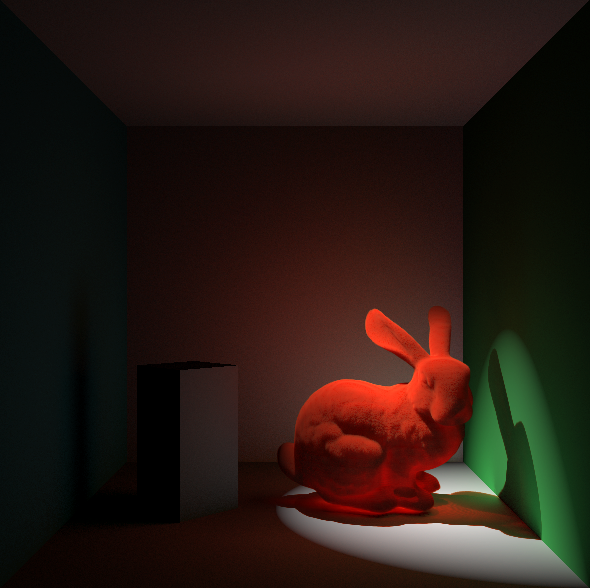
\includegraphics[width=80mm]{../img/ketchup_good_corrected}\\
    }

\end{frame}




%%-----------------------------------------------------------------  CONCLUSION
\begin{frame}[c]{}

    {\centering
    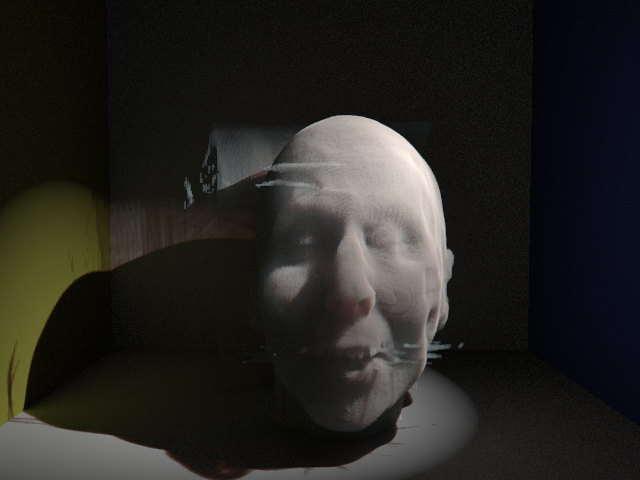
\includegraphics[width=100mm]{../img/face1}\\
    }

\end{frame}




%%-----------------------------------------------------------------  CONCLUSION
\begin{frame}[c]{}

    {\centering
    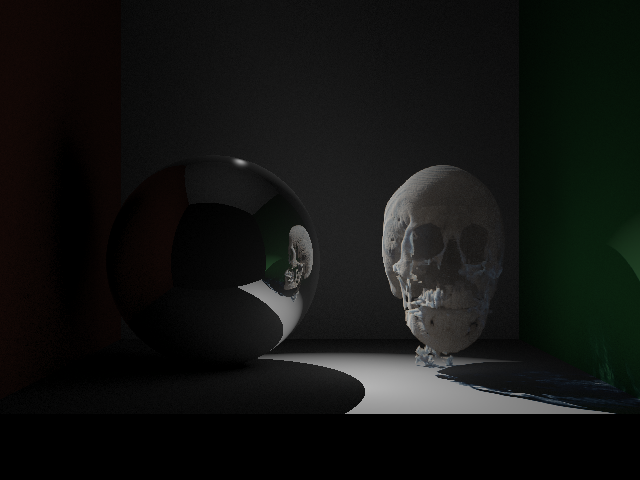
\includegraphics[width=100mm]{../img/sphere_skull}\\
    }

\end{frame}




%%-----------------------------------------------------------------  CONCLUSION
\begin{frame}[c]{}

    {\centering
    \includegraphics[width=80mm]{../img/bunny_glow}\\
    }

\end{frame}




%%-----------------------------------------------------------------  CONCLUSION
\begin{frame}[c]{}

    {\centering
    \includegraphics[width=80mm]{../img/two_sphere_indir}\\
    }

\end{frame}




%%-----------------------------------------------------------------  CONCLUSION
\begin{frame}[c]{}

    {\centering
    \includegraphics[width=80mm]{../img/one_side_corrected}\\
    }

\end{frame}




\section{Concluding Remarks}
\subsection{Works}
%%--------------------------------------------------------------------  RESULTS
\begin{frame}{Future Work}

    \begin{enumerate}
        \item Multiple bounce
        \item Phase functions for volumes
        \item Parallelism
        \item Optimal Sampling
        \item GPU Acceleration
    \end{enumerate}

\end{frame}




\subsection{Final Remarks}
%%-----------------------------------------------------------------  CONCLUSION
\begin{frame}{Conclusion}

    \begin{columns}
        \begin{column}{0.5\textwidth}

            Modifications can be made to PCB to incorporate volume light contributions\\
            \vspace{8mm}

            Even simple implementations show great improvements in performance, nearly ten times faster than traditional Monte Carlo\\
            \vspace{8mm}

            Image quality is comparable to Monte Carlo results

        \end{column}
        \begin{column}{0.5\textwidth}
            \includegraphics[width=\textwidth]{../img/compare}\\
            {\centering\scriptsize PBCEX \textit{(left)} vs Monte Carlo \textit{(right)} \\}
        \end{column}
    \end{columns}

\end{frame}

\end{document}
